\chapter{Elastic rod : equilibrium approach}

\section{Introduction}
Ici on explique que l'approche par les équations d'équilibre est beaucoup plus directe que l'approche énergétique.

\subsection{Goals and contribution}
Dans ce chapitre, après un bref rappel sur le cadre mathématique d'étude des courbes paramétrique de l'espace, on présente les notions de courbures et de torsion géométrique associées au repère de fraient. On montre ensuite le cas plus général d'un repère mobile quelconque attaché à une courbe gamma. On définit enfin la particularité d'un repère mobile adapté à un courbe, et on présente, en sus du repère de Frenet, une approche différente pour accrocher des repères le long d'une courbe (Bishop / RMF / Zéro-twisting frame)

Ici il faudrait préciser la terminologie des auteurs / équations / hypothèses :
Euler-Bernoulli, Navier-Bernoulli, Kirchhoff, Love, Clebesh, Cosserat, Vlassov

\subsection{Related work}
On peu s'instruire dans la publi de Dill \cite{Dill1992}.
Regarder en particulier le premier chapitre de l'HDR de Neukirch \cite{Neukirch2009}.
Regarder également la chronologie des modèles proposée dans la thèse de Theetten \cite{Theetten2007}.
Pourquoi pas proposer une frise chronologique + un tableau de synthèse des hyptohèses.

\cite{Dill1992}
\citet{Neukirch2009}
\cite{Adriaenssens1999}
\cite{Hoogenboom2006}
\cite{Lang2009}
\cite{Spillmann2008}
\cite{Antman2005}

\cite{Neukirch2009} : p69 - \cite{Dill1992} : p16

\subsection{Overview}
Résumé du chapitre


\section{Dynamic Kirchhoff equations}

Writing the balance of linear and angular momentum of a beam slice of infinitesimal yields to the dynamic Kirchhoff equations for a slender beam. An extensive proof of this development is available in \cite{Dill1992}.

\footnote{\blockcquote[p.5]{Dill1992}{The principal normal, binormal, and torsion of the axis, viewed as an element of a space curve, have no special significance in the theory of rods. Use of those special directions as base vectors does not simplify the theory and can mislead the reader into attributing significance to them when none exists. In particular, the curvature of the rod should not be confused with the curvature of the space curve which the axis forms.}}

\begin{figure}[t]
	\centering
	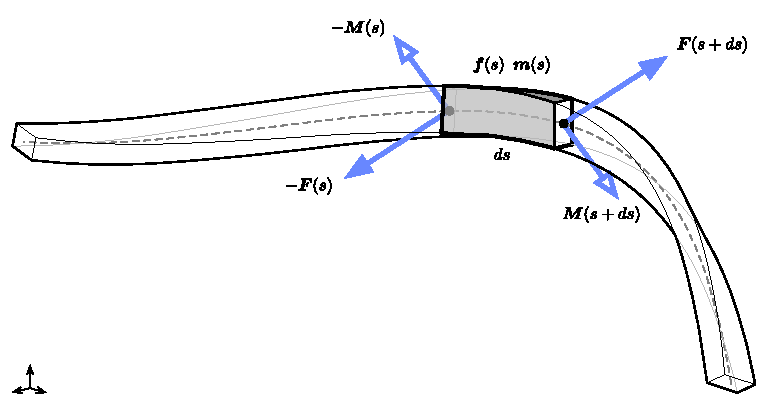
\includegraphics[]{kirchhoff_law.pdf}
	\caption{Internal forces ($\vect{F}$) and moments ($\vect{M}$) acting on an infinitesimal beam slice of length $ds$. The beam is also subject to distributed external forces ($\vect{f}$) and moments ($\vect{m}$).} By convention, internal forces and moments are forces and moments applied by the right part to the left part of the beam.
	\label{fig:5_0}
\end{figure}

\subsection{Balance of linear momentum}
On fait un bilan sur une tranche d'épaisseur $ds$, de centre de gravité $G$ positionné en $\vect{x}_G$ :
\begin{equation}
	\vect{F}(s+ds)-\vect{F}(s) + \vect{f}(s)ds = \left(\frac{\partial \vect{F}}{\partial s}(s)+\vect{f}(s)\right)ds = (\rho Sds)\ddot{\vect{x}}_G
\end{equation}
Which leads to the first equation of Kirchhoff law :
\begin{equation}
	\frac{\partial \vect{F}}{\partial s}+\vect{f} = \rho S \ddot{\vect{x}}_G
\end{equation}

\subsection{Balance of angular momentum}
On fait un bilan sur une tranche d'épaisseur $ds$, de centre de gravité $G$ positionné en $\vect{x}_G$. On applique le théorème du moment cinétique dans un référentiel inertiel :
\begin{equation}
	\begin{aligned}
		\frac{d}{dt}(dI_G) &=
		\vect{M}(s+ds)-\vect{M}(s) + \vect{m}(s)ds
		+ (\tfrac{1}{2}ds\vect{x}')\times \vect{F}(s+ds) + (-\tfrac{1}{2}ds\vect{x}')\times -\vect{F}(s)\\
		&= \left(\frac{\partial \vect{M}}{\partial s}(s)+\vect{m}(s) + \vect{x}'\times \vect{F}(s)\right)ds
	\end{aligned}
\end{equation}
L'évolution temporelle des vecteurs matériels est cette fois décrite par un vecteur de Darboux temporel noté $\vect{\Lambda}$ tel que :
\begin{equation}
	\dot{\vect{d}_{i}}(s) =\vect{\Lambda}(t) \times \vect{d}_i(s)	\quad,\quad
	\vect{\Lambda}(t)
	=
	\begin{bmatrix}
		\Lambda_3(t) \\
		\Lambda_1(t) \\
		\Lambda_2(t)
	\end{bmatrix}
\end{equation}
Les lois de composition / dérivation de la mécanique nous permettent décrire :
\begin{equation}
	\begin{aligned}
		\frac{d}{dt}(dI_G) &= dI_G\dot{\vect{\Lambda}} + \vect{\Lambda}\times dI_G
	\end{aligned}
\end{equation}
Qu'est ce qu'on met dans $dI_G$ ? Et bien tout simplement l'opérateur d'inertie de la section, qui s'exprime à l'aide des moments quadratiques des directions principales de la façon suivante, dans la base des directions principales d'inertie au premier ordre en $ds$ :
\begin{equation}
	dI_G =
	 \begin{bmatrix}
			dI_{G3} & 0 & 0 \\
			0 & dI_{G1} & 0 \\
			0 & 0 & dI_{G2}
	\end{bmatrix}
	\simeq \rho ds
		\begin{bmatrix}
			I_1 + I_2 & 0 & 0 \\
			0 & I_1 & 0 \\
			0 & 0 & I_2
		\end{bmatrix}
\end{equation}
Where :
\begin{subequations}
	\begin{align}
		dI_{G3} &= \int_V \rho (x_1^2+ x_2^2)\;dV
		\simeq \rho ds \int_V (x_1^2+x_2^2)\;dx_1dx_2
		\simeq \rho ds (I_1 + I_2)
		\\
		dI_{G1} &= \int_V \rho (x_2^2+ x_3^2)\;dV
		\simeq \rho ds \int_V x_2^2\;dx_1dx_2
		\simeq \rho ds I_1
		\\
		dI_{G2} &= \int_V \rho (x_1^2+ x_3^2)\;dV
		\simeq \rho ds \int_V x_1^2\;dx_1dx_2
		\simeq \rho ds I_2
	\end{align}
\end{subequations}
Et l'on peut alors écrire la seconde loi de Kirchhoff sous la forme suivante :
\begin{equation}
	\begin{aligned}
		\frac{\partial \vect{M}}{\partial s}(s)+\vect{m}(s) + \vect{x}'\times \vect{F}(s)
		= \rho
			\begin{bmatrix}
				(I_1 + I_2)\dot{\Lambda}_3 + (I_2 - I_1)\Lambda_1\Lambda_2&\\
				I_1 (\dot{\Lambda}_1 + \Lambda_2 \Lambda_3) &\\
				I_2 (\dot{\Lambda}_2 - \Lambda_3 \Lambda_1) &
			\end{bmatrix}
	\end{aligned}
\end{equation}
On montre ensuite :
\begin{equation}
\begin{cases}
&\dot{\vect{d}_3} 	= \vect{\Lambda}\times \vect{d}_3\
				= \Lambda_2\vect{d_1} - \Lambda_1\vect{d_2}\\
&\dot{\vect{d}_1} 	= \vect{\Lambda}\times \vect{d}_1\
				= -\Lambda_2\vect{d_3} + \Lambda_3\vect{d_2}\\
&\dot{\vect{d}_2} 	= \vect{\Lambda}\times \vect{d}_2\
				= \Lambda_1\vect{d_3} - \Lambda_3\vect{d_1}\\
\end{cases}
\quad\Rightarrow\quad
\begin{cases}
&\ddot{\vect{d}_3} 	= \dot{\Lambda}_2\vect{d_1} - \dot{\Lambda}_1\vect{d_2}
				+ \vect{\Lambda} \times \dot{\vect{d}_3}\\
&\ddot{\vect{d}_1} 	= -\dot{\Lambda}_2\vect{d_3} + \dot{\Lambda}_3\vect{d_2}
				+ \vect{\Lambda} \times \dot{\vect{d}_1}\\
&\ddot{\vect{d}_2} 	= \dot{\Lambda}_1\vect{d_3} - \dot{\Lambda}_3\vect{d_1}
				+ \vect{\Lambda} \times \dot{\vect{d}_2}
\end{cases}
\end{equation}
On en déduit en remarquant que $(\vect{\Lambda}\times\dot{\vect{d}_i})\times\vect{d}_i = \Lambda_i(\vect{\Lambda}\times\dot{\vect{d}_i})$ que :
\begin{equation}
\begin{cases}
&\ddot{\vect{d}_3}\times\vect{d}_3
			= (\dot{\Lambda}_2\vect{d_1} - \dot{\Lambda}_1\vect{d_2}
				+ \vect{\Lambda} \times \dot{\vect{d}_3}) \times \vect{d}_3
			= (- \dot{\Lambda}_1 + \Lambda_2\Lambda_3)\vect{d}_1
			-(\dot{\Lambda}_2 + \Lambda_1\Lambda_3)\vect{d}_2\\
&\ddot{\vect{d}_1}\times\vect{d}_1
			= -\dot{\Lambda}_2\vect{d_3} + \dot{\Lambda}_3\vect{d_2}
				+ \vect{\Lambda} \times \dot{\vect{d}_1} \times \vect{d}_1
			= -(\dot{\Lambda}_3 + \Lambda_1\Lambda_2)\vect{d}_3
			+(-\dot{\Lambda}_2 + \Lambda_1\Lambda_3)\vect{d}_2\\
&\ddot{\vect{d}_2} \times\vect{d}_2
			= \dot{\Lambda}_1\vect{d_3} - \dot{\Lambda}_3\vect{d_1}
				+ \vect{\Lambda} \times \dot{\vect{d}_2}  \times \vect{d}_2
			= (- \dot{\Lambda}_3 + \Lambda_1\Lambda_2)\vect{d}_3
			-(\dot{\Lambda}_1 + \Lambda_2\Lambda_3)\vect{d}_1\\
\end{cases}
\end{equation}
On peut alors conclure sur l'expression de l'equation de kirchoff :
\begin{equation}
	\frac{\partial \vect{M}}{\partial s}(s)+\vect{m}(s) + \vect{d}_3'\times \vect{F}(s) = I_1\vect{d}_1 \times \ddot{\vect{d}_1} + I_2 \vect{d}_2 \times \ddot{\vect{d}_2}
\end{equation}

\section{Equations of motion}
\subsection{Constitutive equations}

Attention, pas d'effort normal par loi constitutive en principe car on est dans un modèle inextensible.
L'effort normal est calculé par la loi d'équilibre avec les moments et/ou efforts tranchants.
Ici, on postulera tout de même une telle loi constitutive pour la résolution numérique. Ce qui nous amène à considérer une tige quasiment inextensible.

\note{
point à creuser. en gros je suis entrain de dire que dans le modèle classique à 3DOF type Douthe ou Barnes, il n'est pas nécessaire d'introduire la raideur axiale (mais alors où intervient la section ?). L'effort normal est déduit des équations d'équilibre.

En fait cela ne semble pas possible. Il faaut alors revenir à l'équation constitutive qui donne l'effort normal, mais alors quid de l'hypothèse quasistatique ?

Dans le fond, l'hyptohèse d'inextensibilité c'est dire que les déformations axiales sont négligeable devant les autres modes de déformation (flexion et/ou torsion).
Mais pour caractériser l'effort normal lui même, il faut bien considérer une élongation.

Ou alors, peut-être qu'il faut comprendre que l'effort normal est déduit uniquement des conditions aux limites et/ou éventuellement des efforts extérieurs appliqués à la centerline.

Pour comprendre le traitement de l'inextensibilité, regarder \cite{Antman2005} p50.
Qu'apporte l'hypothèse d'inextensibilité. Est-elle raisonnable. Tps de calcul par rapport au cas extensible.
}

\begin{subequations}
	\begin{align}
		\vect{N} &= ES(\|\vect{d}_3'\|-\|\overbar{\vect{d}_3}'\|)\vect{d}_3
		\\
		\vect{M_1} &= EI_1(\kappa_1-\overbar{\kappa_1})\vect{d}_1
		\\
		\vect{M_2} &= EI_2(\kappa_2-\overbar{\kappa_2})\vect{d}_2
		\\
		\vect{Q} &= [GJ(\theta'-\overbar{\theta}') - EC_w(\theta'''-\overbar{\theta}''')]\vect{d}_3
	\end{align}
\end{subequations}


\subsection{Internal forces and moments}

Efforts internes de coupure :
\begin{subequations}
	\begin{align}
		\vect{F}_{int} &= N\vect{d}_3 + T_1\vect{d}_1 + T_2\vect{d}_2
		\\
		\vect{M}_{int} &= Q\vect{d}_3 + M_1\vect{d}_1 + M_2\vect{d}_2
	\end{align}
\end{subequations}

Efforts externes appliqués linéiques :
\begin{subequations}
	\begin{align}
		\vect{f}_{ext} &= f_3\vect{d}_3 + f_1\vect{d}_1 + f_2\vect{d}_2
		\\
		\vect{m}_{ext} &= m_3\vect{d}_3 + m_1\vect{d}_1 + m_2\vect{d}_2
	\end{align}
\end{subequations}

\subsection{Rod dynamic}

First Kirchhoff law projecting on the material frame basis :
\begin{subequations}
	\begin{align}
		N' + \kappa_1 T_2 - \kappa_2 T_1 + f_3 &= \rho S \ddot{x_3}
		\\
		T_1' + \kappa_2 N - \tau T_2 + f_1 &= \rho S \ddot{x_1}
		\\
		T_2' - \kappa_1 N + \tau T_1 + f_2 &= \rho S \ddot{x_2}
	\end{align}
\end{subequations}
Second Kirchhoff law projecting on the material frame basis :
\begin{subequations}
	\begin{align}
		Q' + \kappa_1 M_2 - \kappa_2 M_1 + m_3 &= (I_1 + I_2)\dot{\Lambda}_3 + (I_2 - I_1)\Lambda_1\Lambda_2
		\label{eq:3_16_a}\\
		M_1' + \kappa_2 Q - \tau M_2 - T_2 + m_1 &= I_1 (\dot{\Lambda}_1 + \Lambda_2 \Lambda_3)
		\label{eq:3_16_b}\\
		M_2' - \kappa_1 Q + \tau M_1 + T_1 + m_2 &= I_2 (\dot{\Lambda}_2 - \Lambda_3 \Lambda_1)
		\label{eq:3_16_c}
	\end{align}
\end{subequations}

\section{Geometric interpretation}

Ici, on peut mettre l'interprétation géométrique (cf pdf LDP notes).
Cela consiste essentiellement à 2/3 schémas bien pensés à produire + à écrire les projections au 1er ordre.

\begin{figure}[t]
	\centering
	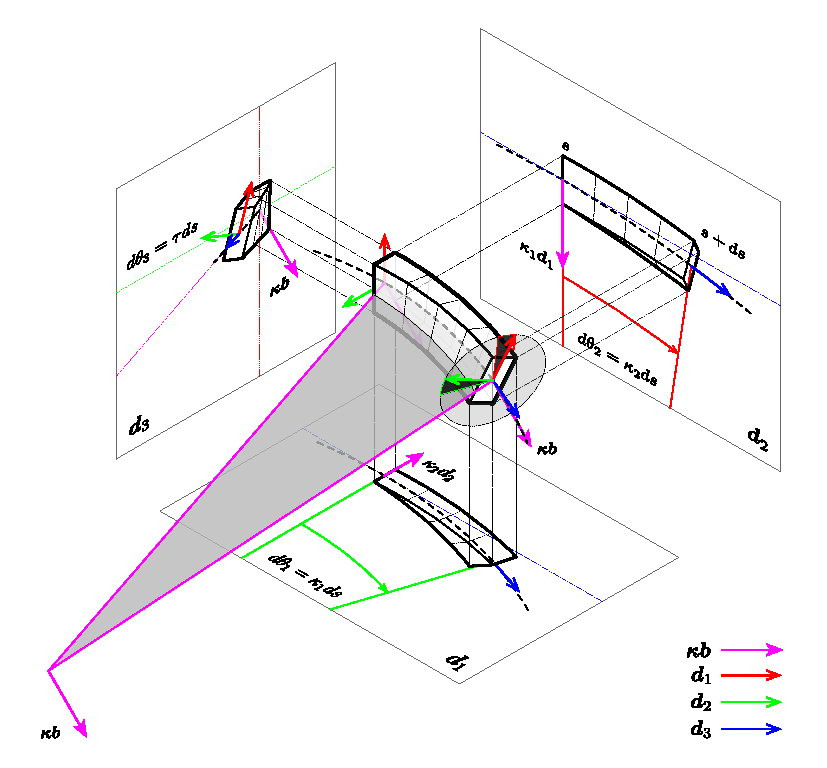
\includegraphics[]{kirchhoff_geometry.pdf}
	\caption{Osculating circles for a spiral curve at different parameters.}
	\label{fig:5}
\end{figure}

%\begin{figure}[H]
%	\captionsetup[subfloat]{captionskip=10pt}
%     	\centering
%     	\subfloat[][Infinitesimal deformation.]{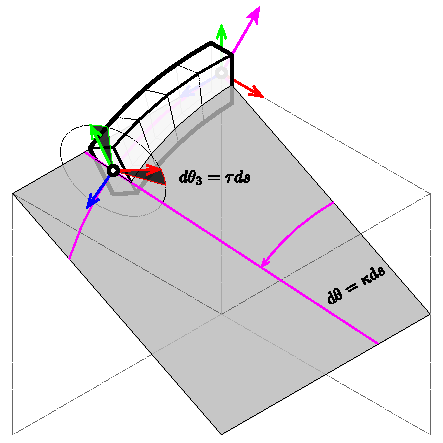
\includegraphics{kirchhoff_geometry_kb.pdf}\label{<figure1>}} \\
%	\subfloat[][Contribution of the internal force.]{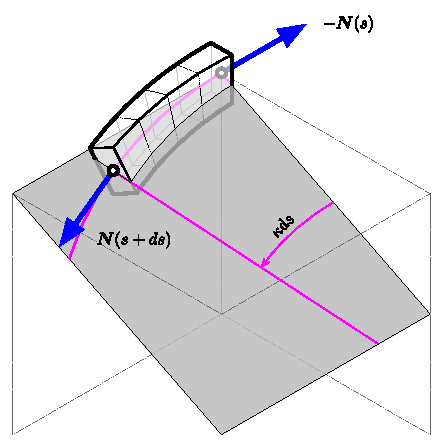
\includegraphics{kirchhoff_balance_T_kb.pdf}\label{<figure1>}}
%	\subfloat[][Contribution of the internal moment.]{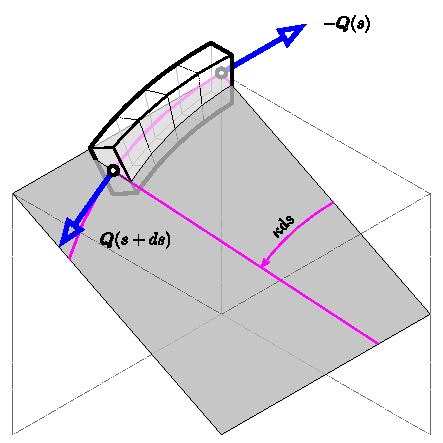
\includegraphics{kirchhoff_balance_M_kb.pdf}\label{<figure2>}}
%	\vspace{10pt}
%	\caption{Projection of the static equilibrium equations in the plane normal to $\kappa\vect{b}$.}
%     \label{fig:5_2}
%\end{figure}

%\begin{figure}[H]
%	\captionsetup[subfloat]{captionskip=10pt}
%     	\centering
%     	\subfloat[][Infinitesimal deformation.]{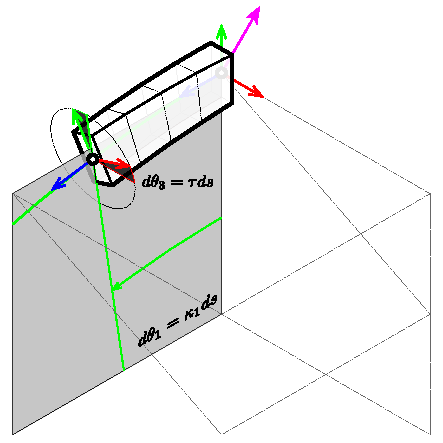
\includegraphics{kirchhoff_geometry_d1.pdf}\label{<figure1>}} \\
%	\subfloat[][Contribution of the internal force.]{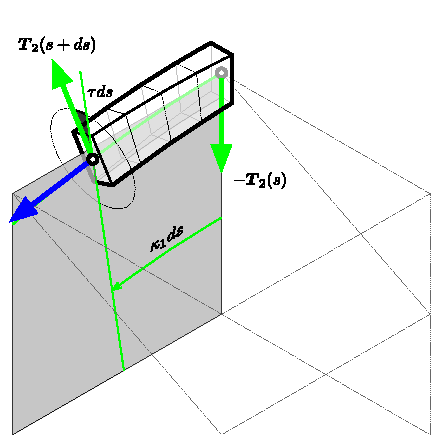
\includegraphics{kirchhoff_balance_T_d1.pdf}\label{<figure1>}}
%	\subfloat[][Contribution of the internal moment.]{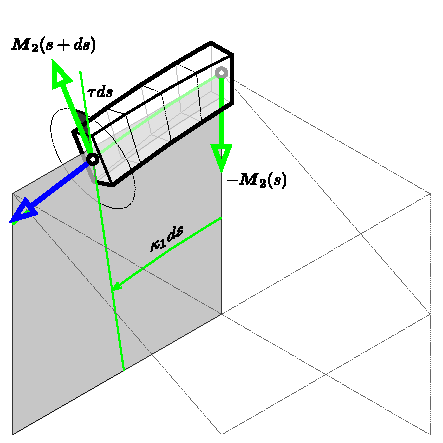
\includegraphics{kirchhoff_balance_M_d1.pdf}\label{<figure2>}}
%	\vspace{10pt}
%	\caption{Projection of the static equilibrium equations in the plane normal to $\vect{d}_1$.}
%     \label{fig:5_2}
%\end{figure}
%
%\begin{figure}[H]
%	\captionsetup[subfloat]{captionskip=10pt}
%     	\centering
%     	\subfloat[][Infinitesimal deformation.]{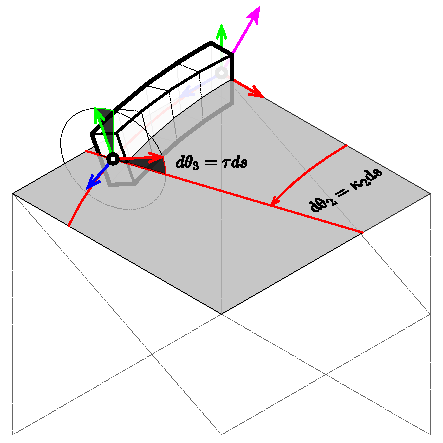
\includegraphics{kirchhoff_geometry_d2.pdf}\label{<figure1>}} \\
%	\subfloat[][Contribution of the internal force.]{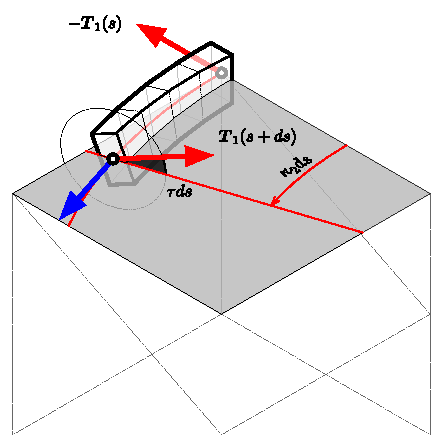
\includegraphics{kirchhoff_balance_T_d2.pdf}\label{<figure1>}}
%	\subfloat[][Contribution of the internal moment.]{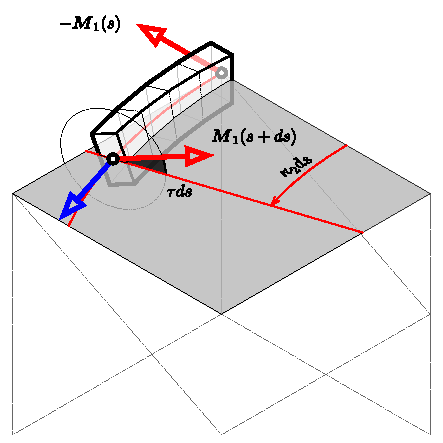
\includegraphics{kirchhoff_balance_M_d2.pdf}\label{<figure2>}}
%	\vspace{10pt}
%	\caption{Projection of the static equilibrium equations in the plane normal to $\vect{d}_2$.}
%     \label{fig:5_2}
%\end{figure}

% ============
 
\begin{figure}[p]
  \begin{leftfullpage}
    \captionsetup[subfloat]{captionskip=10pt}
     	\centering
     	\subfloat[][Infinitesimal deformation.]{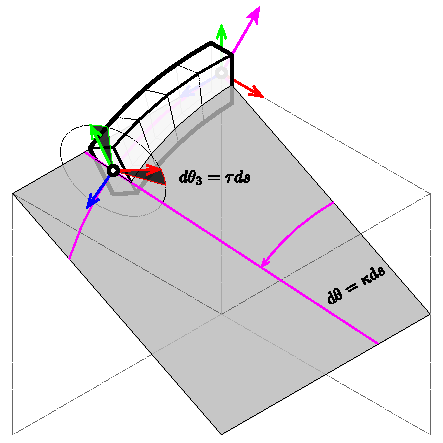
\includegraphics{kirchhoff_geometry_kb.pdf}\label{fig:5_2_a}} \\
	\vspace{30pt}
	\subfloat[][Contributions of the internal forces.]{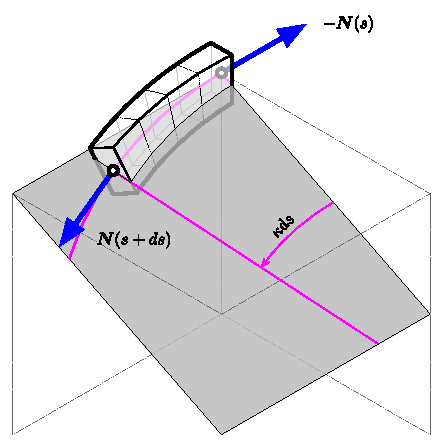
\includegraphics{kirchhoff_balance_T_kb.pdf}\label{fig:5_2_b}}
	\subfloat[][Contributions of the internal moments.]{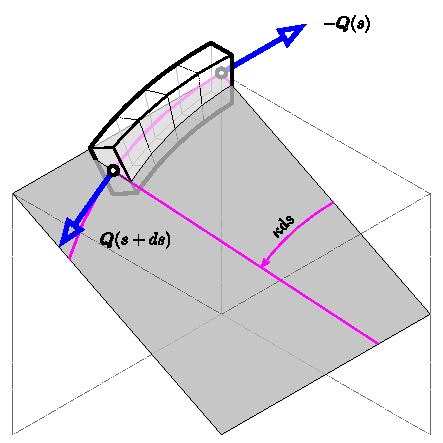
\includegraphics{kirchhoff_balance_M_kb.pdf}\label{fig:5_2_c}}
	\vspace{30pt}
	\caption{Influence of the centerline curvature ($\kappa$) in the deviation of internal forces and moments along the centerline.}     
	\label{fig:5_2}
 \end{leftfullpage}
\end{figure}
\begin{figure}[p]
	\begin{fullpage}
	\subsubsection{Contributions to the balance of forces}
	\vspace{10pt}
	$\vect{N}(s+ds)$ is deviated from $\vect{d}_3(s)$ by an angle $d\theta = \kappa ds$ along $ds$ (\cref{fig:5_2_b}). Thus, its overall contribution to the balance of forces over $\vect{d}_3(s)$ is : 
	\begin{equation*}
		N(s+ds) \cos(\kappa ds) - N(s) = N'(s) ds + o(ds)
	\end{equation*}	
	\vspace{10pt}
	\subsubsection{Contributions to the balance of moments}
	\vspace{10pt}
	$\vect{Q}(s+ds)$ is deviated from $\vect{d}_3(s)$ by an angle $d\theta = \kappa ds$ along $ds$ (\cref{fig:5_2_c}). Thus, its overall contribution to the balance of moments over $\vect{d}_3(s)$ is : 
	\begin{equation*}
		Q(s+ds) \cos(\kappa ds) - Q(s) = Q'(s) ds + o(ds)
	\end{equation*}	
	  \end{fullpage}
\end{figure}

% ============
 
\begin{figure}[p]
  \begin{leftfullpage}
    \captionsetup[subfloat]{captionskip=10pt}
     	\centering
     	\subfloat[][Infinitesimal deformation.]{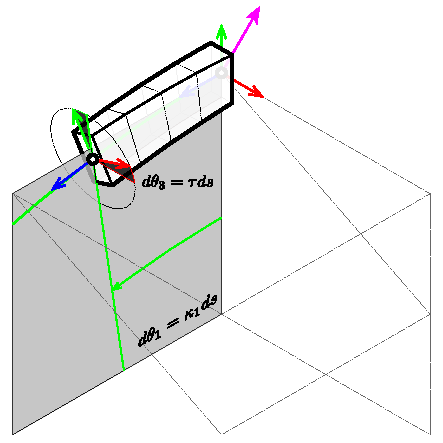
\includegraphics{kirchhoff_geometry_d1.pdf}\label{fig:5_3_a}} \\
	\vspace{30pt}
	\subfloat[][Contributions of the internal forces.]{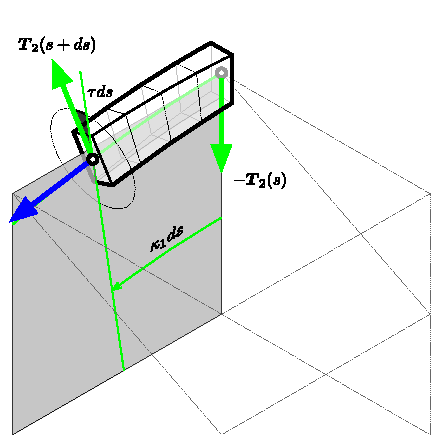
\includegraphics{kirchhoff_balance_T_d1.pdf}\label{fig:5_3_b}}
	\subfloat[][Contributions of the internal moments.]{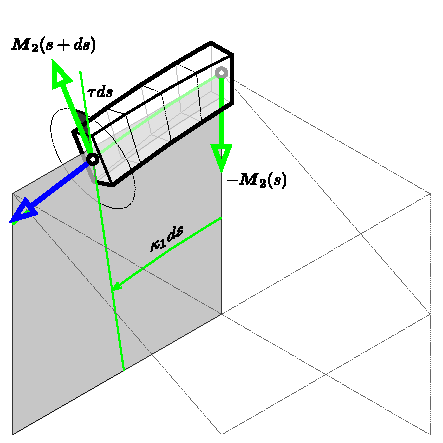
\includegraphics{kirchhoff_balance_M_d1.pdf}\label{fig:5_3_c}}
	\vspace{30pt}
	\caption{Influence of the first material curvature ($\kappa_1$) in the deviation of internal forces and moments along the centerline.}     
	\label{fig:5_3}
 \end{leftfullpage}
\end{figure}
\begin{figure}[p]
	\begin{fullpage}
	\subsubsection{Contributions to the balance of forces}
	\vspace{10pt}
	
	$\vect{T}_2(s+ds)$ is deviated from $\vect{d}_2(s)$ by the combined angles $d\theta_3 = \tau ds$ and $d\theta_2 = \kappa_2 ds$ along $ds$ (\cref{fig:5_3_b}). Thus, its overall contribution to the balance of forces over $\vect{d}_1(s)$ is : 
	\begin{equation*}
		-T_2(s+ds) \sin(\tau ds) \cos(\kappa_2 ds) = -\tau T_2(s) ds + o(ds)
	\end{equation*}	
	
	$\vect{T}_2(s+ds)$ is deviated from $\vect{d}_2(s)$ by the combined angles $d\theta_3 = \tau ds$ and $d\theta_1 = \kappa_1 ds$ along $ds$ (\cref{fig:5_3_b}). Thus, its overall contribution to the balance of forces over $\vect{d}_2(s)$ is : 
	\begin{equation*}
		-T_2(s) + T_2(s+ds) \cos(\tau ds) \cos(\kappa_1 ds) = T'_2 (s) ds + o(ds)
	\end{equation*}	
	
	$\vect{T}_2(s+ds)$ is deviated from $\vect{d}_2(s)$ by the combined angles $d\theta_3 = \tau ds$ and $d\theta_1 = \kappa_1 ds$ along $ds$ (\cref{fig:5_3_b}). Thus, its overall contribution to the balance of forces over $\vect{d}_3(s)$ is : 
	\begin{equation*}
		T_2(s+ds) \cos(\tau ds) \sin(\kappa_1 ds) = \kappa_1 T_2(s) ds + o(ds)
	\end{equation*}
		
	$\vect{N}(s+ds)$ is deviated from $\vect{d}_3(s)$ by the combined angles $d\theta_2 = \kappa_2 ds$ and $d\theta_1 = \kappa_1 ds$ along $ds$ (\cref{fig:5_3_b}). Thus, its overall contribution to the balance of forces over $\vect{d}_2(s)$ is : 
	\begin{equation*}
		-N(s+ds) \cos(\kappa_2 ds) \sin(\kappa_1 ds) = -\kappa_1 N(s) ds + o(ds)
	\end{equation*}	
	\vspace{10pt}

	\subsubsection{Contributions to the balance of moments}
	\vspace{10pt}
	
	$\vect{T}_2(s+ds)$ is deviated from the plane normal to $\vect{d}_1(s)$ by the angle $d\theta_3 = \tau ds$ along $ds$ (\cref{fig:5_3_b}). It produces a moment around $\vect{d}_1$ with the lever arm $b =  \cos(\kappa_2 ds) ds$. Thus, its overall contribution to the balance of moments over $\vect{d}_1(s)$ is : 
	\begin{equation*}
		-T_2(s+ds) \cos(\tau ds) (\cos(\kappa_2 ds) ds) = -T_2(s) ds + o(ds)
	\end{equation*}
	
	$\vect{M}_2(s+ds)$ is deviated from $\vect{d}_2(s)$ by the combined angles $d\theta_3 = \tau ds$ and $d\theta_2 = \kappa_2 ds$ along $ds$ (\cref{fig:5_3_c}). Thus, its overall contribution to the balance of moments over $\vect{d}_1(s)$ is : 
	\begin{equation*}
		-M_2(s+ds) \sin(\tau ds) \cos(\kappa_2 ds) = -\tau M_2 (s) ds + o(ds)
	\end{equation*}	
	
	$\vect{M}_2(s+ds)$ is deviated from $\vect{d}_2(s)$ by the combined angles $d\theta_3 = \tau ds$ and $d\theta_1 = \kappa_1 ds$ along $ds$ (\cref{fig:5_3_c}). Thus, its overall contribution to the balance of moments over $\vect{d}_2(s)$ is : 
	\begin{equation*}
		-M_2(s) + M_2(s+ds) \cos(\tau ds) \cos(\kappa_1 ds) = M'_2 (s) ds + o(ds)
	\end{equation*}
	
	$\vect{M}_2(s+ds)$ is deviated from $\vect{d}_2(s)$ by the combined angles $d\theta_3 = \tau ds$ and $d\theta_1 = \kappa_1 ds$ along $ds$ (\cref{fig:5_3_c}). Thus, its overall contribution to the balance of moments over $\vect{d}_3(s)$ is : 
	\begin{equation*}
		M_2(s+ds) \cos(\tau ds) \sin(\kappa_1 ds) = \kappa_1 M_2 (s) ds + o(ds)
	\end{equation*}	
	
	$\vect{Q}(s+ds)$ is deviated from $\vect{d}_3(s)$ by the combined angles $d\theta_2 = \kappa_2 ds$ and $d\theta_1 = \kappa_1 ds$ along $ds$ (\cref{fig:5_3_c}). Thus, its overall contribution to the balance of moments over $\vect{d}_2(s)$ is : 
	\begin{equation*}
		-Q(s+ds) \cos(\kappa_2 ds) \sin(\kappa_1 ds) = -\kappa_1 Q(s) ds + o(ds)
	\end{equation*}	
	  \end{fullpage}
\end{figure}

% ============
 
\begin{figure}[p]
  \begin{leftfullpage}
    \captionsetup[subfloat]{captionskip=10pt}
     	\centering
     	\subfloat[][Infinitesimal deformation.]{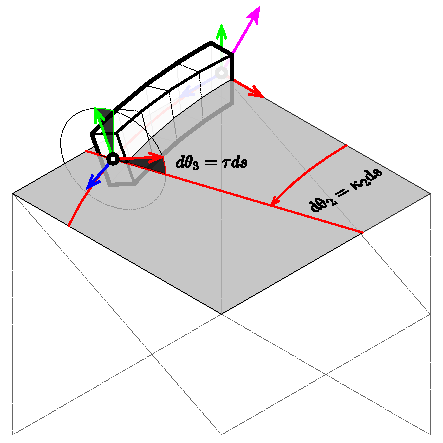
\includegraphics{kirchhoff_geometry_d2.pdf}\label{fig:5_4_a}} \\
	\vspace{30pt}
	\subfloat[][Contributions of the internal forces.]{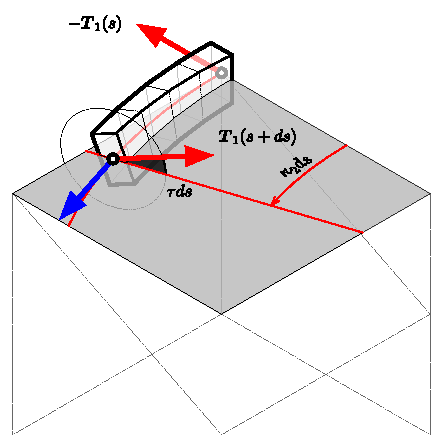
\includegraphics{kirchhoff_balance_T_d2.pdf}\label{fig:5_4_b}}
	\subfloat[][Contributions of the internal moments.]{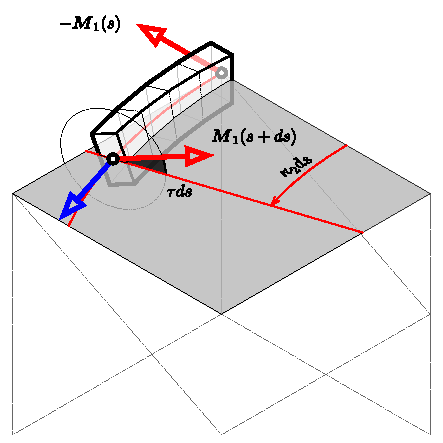
\includegraphics{kirchhoff_balance_M_d2.pdf}\label{fig:5_4_c}}
	\vspace{30pt}
	\caption{Influence of the second material curvature ($\kappa_2$) in the deviation of internal forces and moments along the centerline.}     
	\label{fig:5_4}
 \end{leftfullpage}
\end{figure}
\begin{figure}[p]
	\begin{fullpage}
	\subsubsection{Contributions to the balance of forces}
	\vspace{10pt}
	
	$\vect{T}_1(s+ds)$ is deviated from $\vect{d}_1(s)$ by the combined angles $d\theta_3 = \tau ds$ and $d\theta_2 = \kappa_2 ds$ along $ds$ (\cref{fig:5_4_b}). Thus, its overall contribution to the balance of forces over $\vect{d}_1(s)$ is : 
	\begin{equation*}
		-T_1(s) + T_1(s+ds) \cos(\tau ds) \cos(\kappa_2 ds) = T'_1 (s) ds + o(ds)
	\end{equation*}
	
	$\vect{T}_1(s+ds)$ is deviated from $\vect{d}_1(s)$ by the combined angles $d\theta_3 = \tau ds$ and $d\theta_1 = \kappa_1 ds$ along $ds$ (\cref{fig:5_4_b}). Thus, its overall contribution to the balance of forces over $\vect{d}_2(s)$ is : 
	\begin{equation*}
		T_1(s+ds) \sin(\tau ds) \cos(\kappa_1 ds) = \tau T_1 (s) ds + o(ds)
	\end{equation*}	
	
	$\vect{T}_1(s+ds)$ is deviated from $\vect{d}_1(s)$ by the combined angles $d\theta_3 = \tau ds$ and $d\theta_2 = \kappa_2 ds$ along $ds$ (\cref{fig:5_4_b}). Thus, its overall contribution to the balance of forces over $\vect{d}_3(s)$ is : 
	\begin{equation*}
		-T_1(s+ds) \cos(\tau ds) \sin(\kappa_2 ds) = - \kappa_2 T_1(s) ds + o(ds)
	\end{equation*}	
	
	$\vect{N}(s+ds)$ is deviated from $\vect{d}_3(s)$ by the combined angles $d\theta_1 = \kappa_1 ds$ and $d\theta_2 = \kappa_2 ds$ along $ds$ (\cref{fig:5_4_b}). Thus, its overall contribution to the balance of forces over $\vect{d}_1(s)$ is : 
	\begin{equation*}
		N(s+ds) \cos(\kappa_1 ds) \sin(\kappa_2 ds) = \kappa_2 N(s) ds + o(ds)
	\end{equation*}	
	\vspace{10pt}
	
	\subsubsection{Contributions to the balance of moments}
	\vspace{10pt}
	
		$\vect{T}_1(s+ds)$ is deviated from the plane normal to $\vect{d}_2(s)$ by the angle $d\theta_3 = \tau ds$ along $ds$ (\cref{fig:5_4_b}). It produces a moment around $\vect{d}_2$ with the lever arm $b =  \cos(\kappa_1 ds) ds$. Thus, its overall contribution to the balance of moments over $\vect{d}_2(s)$ is : 
	\begin{equation*}
		T_1(s+ds) \cos(\tau ds) (\cos(\kappa_1 ds) ds) = T_1(s) ds + o(ds)
	\end{equation*}
	
	$\vect{M}_1(s+ds)$ is deviated from $\vect{d}_1(s)$ by the combined angles $d\theta_3 = \tau ds$ and $d\theta_2 = \kappa_2 ds$ along $ds$ (\cref{fig:5_4_c}). Thus, its overall contribution to the balance of moments over $\vect{d}_1(s)$ is : 
	\begin{equation*}
		-M_1(s) + M_1(s+ds) \cos(\tau ds) \cos(\kappa_2 ds) = M'_1 (s) ds + o(ds)
	\end{equation*}	
	
	$\vect{M}_1(s+ds)$ is deviated from $\vect{d}_1(s)$ by the combined angles $d\theta_3 = \tau ds$ and $d\theta_2 = \kappa_2 ds$ along $ds$ (\cref{fig:5_4_c}). Thus, its overall contribution to the balance of moments over $\vect{d}_2(s)$ is : 
	\begin{equation*}
		M_1(s+ds) \sin(\tau ds) \cos(\kappa_2 ds) = \tau M_1 (s) ds + o(ds)
	\end{equation*}	
	
	$\vect{M}_1(s+ds)$ is deviated from $\vect{d}_1(s)$ by the combined angles $d\theta_3 = \tau ds$ and $d\theta_2 = \kappa_2 ds$ along $ds$ (\cref{fig:5_4_c}). Thus, its overall contribution to the balance of moments over $\vect{d}_3(s)$ is : 
	\begin{equation*}
		-M_1(s+ds) \cos(\tau ds) \sin(\kappa_2 ds) = -\kappa_2 M_1 (s) ds + o(ds)
	\end{equation*}	
	
	$\vect{Q}(s+ds)$ is deviated from $\vect{d}_3(s)$ by the combined angles $d\theta_1 = \kappa_1 ds$ and $d\theta_2 = \kappa_2 ds$ along $ds$ (\cref{fig:5_4_c}). Thus, its overall contribution to the balance of moments over $\vect{d}_1(s)$ is : 
	\begin{equation*}
		Q(s+ds) \cos(\kappa_1 ds) \sin(\kappa_2 ds) = \kappa_2 Q(s) ds + o(ds)
	\end{equation*}	
	  \end{fullpage}
\end{figure}



\section{Main hypothesis}

On néglige les forces d'inertie liées à la rotation de l'élément  (devant quoi ?? traitement quasi-statique par rapport à la rotation). Cette hypothèse est faite explicitement chez Florence Bertail :

\cite{Casati2013}
\guil{neglecting inertial momentum due to the vanishing cross- section lead to the following dynamic equations for a Kirchhoff rod}

Cette hypothèse est faite mais passée sous silence chez Douthe, Adriaenssen, D'Amico lorsqu'ils déduisent l'effort tranchant du moment de flexion.

Principe :

- les équations constitutives permettent le calcul de $M_1$, $M_2$, $Q$ à partir de la géométrie $\{\vect{x},\theta\}$.

- La seconde loi de kirchhoff projetée sur les axes matériels 1 et 2 de la section me donnent accès aux efforts tranchants $T_1$ et $T_2$.

- La seconde loi de kirchhoff projetée sur les axes matériel 3 (tangente à la centerline) de la section me donnent l"hypothèse quasi-statique de Audoly.

\section{Conclusion}
Remind that the beam is subject to a distributed external force $\vect{f}_{ext}$ and a distributed external moment $\vect{m}_{ext}$.

We neglect rotational inertial effects on $\vect{d}_1$ et $\vect{d}_2$ in \eqref{eq:3_16_b} and \eqref{eq:3_16_c} which leads to the following shear force :
\begin{equation}
	\vect{T}(s) = \vect{d}_3 \times (\vect{M}' + \vect{m}_{ext})
		+ Q \kappa\vect{b} - \tau \vect{M}
\end{equation}
\note{We may neglect as well the last term ($\tau \vect{M}$) and get back to the shear force obtained by the variational approach.} The total internal force acting on the beam is hence given by :
\begin{equation}
	\vect{F}(s) = \vect{N}(s) + \vect{T}(s)
\end{equation}
Sections are subject to the following rotational moment around the centerline :
\begin{equation}
	\begin{aligned}
	\vect{\Gamma}(s) = Q' + \vect{d}_3 \cdot ( \kappa\vect{b} \times \mat{M} + \vect{m}_{ext})
	\end{aligned}
\end{equation}


\bibliographystyle{alpha}
\bibliography{../library}
